\scanpage{14}
c)
\[
\begin{aligned}
\unsure{\mathfrak{S}|\mathcal{S}}_4&\simeq\operatorname{Aff}\,2,\mathbb{F}_2)\simeq\operatorname{GP}(1,\mathbb{F}_3)\\
\unsure{\mathfrak{A}|\mathcal{A}}_4&\simeq\operatorname{Aff}(1,\mathbb{F}_4)\qquad ?
\end{aligned}
\]
% Two detached points at the right of c), between its two formula baselines;
% writing versus surface trace remains uncertain, with no punctuation assigned.
\margin{\figure{\unsure{\begin{tikzpicture}[x=1mm,y=1mm]
\fill (0,1.2) ellipse [x radius=.15,y radius=.19];
\fill[gray] (-.04,0) ellipse [x radius=.13,y radius=.22];
\end{tikzpicture}}}}

d)
\[
\begin{aligned}
\mathfrak{S}_5&\simeq\operatorname{GP}(1,\mathbb{F}_5)\\
\mathfrak{A}_5&\simeq\operatorname{GP}(1,\mathbb{F}_4)
\end{aligned}
\]

Quelques groupes classiques sur un corps $k$

\diagram{\(\left.
\begin{tikzcd}[ampersand replacement=\&,column sep=small,row sep=1em]
1\arrow[r] \& k^*\arrow[r] \& \operatorname{Gl}(V)\arrow[r] \&\operatorname{GP}(V)\arrow[r,dash]\&1\\
1\arrow[r] \& k^*\arrow[r,dash] \&\operatorname{Gl}(n,k)\arrow[r] \&\operatorname{GP}(n-1,k)\arrow[r]\&1
\end{tikzcd}
\right\}\;\text{ne \unsure{splitte} pas en général}\)}

% Left margin note, rising to the right; its surrounding oval has two gaps.
\reversemarginpar
\margin{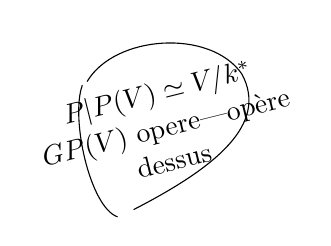
\begin{tikzpicture}[baseline=(proj.base)]
\begin{scope}[rotate=14,transform shape]
\node[inner sep=1pt,align=center] (proj) at (0,0)
 {\shortstack{$\unsure{\mathbb{P}|P}(V)\simeq V/k^*$\\$\operatorname{GP}(V)$ \unsure{opere|opère}\\dessus}};
\draw (-.90,.75) .. controls (-1.15,.38) and (-1.18,-.78) .. (-.87,-.98);
\draw (-.83,.78) .. controls (-.35,1.27) and (.85,1.06) .. (1.10,.40)
 .. controls (1.28,-.30) and (.50,-.67) .. (-.65,-.94);
\end{scope}
\end{tikzpicture}}
\normalmarginpar

\[
\begin{aligned}
\text{Structure de $k$-vectoriel }\quad
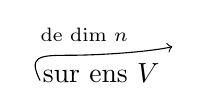
\begin{tikzpicture}[baseline=(sur.base)]
\node[anchor=base west,inner sep=0pt] (sur) at (0,0) {sur ens $V$};
\node[anchor=base west,inner sep=0pt,font=\scriptsize] at (-.03,.52) {\inserted{de dim $n$}};
\draw[->] (-.03,.02) .. controls (-.18,.32) and (-.05,.34) .. (.30,.34)
 .. controls (.85,.34) and (1.45,.40) .. (1.65,.45);
\end{tikzpicture}
&\quad\longleftrightarrow\quad\text{donnée d'\unsure{un|une} \unsure{élemt|élémt|élement|élément}}\\
&\qquad\text{de}\quad\operatorname{Isom}_{\text{ens}}(k^n,V)/\operatorname{Gl}(n,k)
\end{aligned}
\]

Structure de $k$-espace affine de dim $n$ sur \deleted{$E$} ens $E$
\[
\begin{aligned}
&\longleftrightarrow\quad\text{donnée d'un élément de}\\
&\hspace{3em}\operatorname{Isom}_{\text{ens}}(k^n,V)/\operatorname{Aff}(n,k)
\end{aligned}
\]

[ De façon \unsure{générale|général}, \deleted{si $Z$ est un groupe}, la notion de
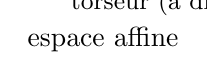
\begin{tikzpicture}[baseline=(oldaff.base)]
\node[anchor=base west,inner sep=0pt] (oldaff) at (0,0) {\deleted{espace affine}};
\node[overlay,anchor=base west,inner sep=0pt,font=\small] at (.55,.48)
 {\inserted{torseur (à droite, disons) $E$}};
\end{tikzpicture}
sous groupe non précisé peut être considéré comme structure sur le seul ens de base $E$,
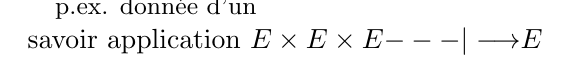
\begin{tikzpicture}[baseline=(oldapp.base)]
\node[anchor=base west,inner sep=0pt] (oldapp) at (0,0)
 {\deleted{\unsure{savoir application} $E\times E\times E\unsure{\mathbin{\text{---}}|\longrightarrow}E$}};
\node[overlay,anchor=base west,inner sep=0pt,font=\small] at (.35,.43)
 {\inserted{p.ex. donnée d'un}};
\end{tikzpicture}
\deleted{$(x,y,z)\unsure{\longmapsto|\mathrel{\vert\! -\! -}}\unsure{6x|sx}$}
couple $\Gamma\subset\mathfrak{S}_{E}$ ss-grpe, tel que \ldots ] ; valable pour ens. à grpe d'op \uline{fidèle}\ldots ]

Une structure d'\uline{espace affine sous} $k$ est alors la donnée d'un tel $\Gamma$, avec \deleted{\unsure{$\Gamma$ com}} comm, \deleted{et} un hom d'anneaux unit.
\[
 k\longrightarrow\operatorname{End}_{\mathbb{Z}}(\Gamma)\quad\ldots\qquad ]
\]

Structure de $k$-espace projectif de dim $n$ sur $\unsure{P|\mathbb P}$
\[
\begin{tikzpicture}[baseline=(projective.base)]
\node[anchor=base west,inner sep=0pt] (projective) at (0,0)
 {$\displaystyle\longleftrightarrow\quad\text{donnée de}\quad
 \operatorname{Isom}_{\text{ens}}\left(
 \underset{\substack{\rotatebox{90}{$=$}\\(k^n-\unsure{(0)|\{0\}|0}/k^*}}{\mathbb{P}^{n-1}(k)},P\right)
 /\operatorname{GP}(n-1,k)$};
% The enclosure over the arrow is open at its top, not a closed box.
\node[inner sep=0pt,font=\small] at (.35,.70) {déf};
\draw (.02,.87) -- (.02,.45) -- (.68,.45) .. controls (.75,.45) and (.75,.64) .. (.75,.86);
\draw[->] (.36,.45) -- (.36,.12);
% Divider bends below the small quotient and continues rightward.
\draw (2.70,-.77) -- (6.00,-.77)
 .. controls (6.35,-.77) and (6.25,-1.17) .. (6.70,-1.17) -- (11.60,-1.17);
\end{tikzpicture}
\]

\diagram{\begin{tikzcd}[ampersand replacement=\&,column sep=small,row sep=.6em]
\operatorname{Gl}(n,k)\arrow[r]\&\operatorname{Aff}(n,k)\arrow[r]\&\operatorname{GP}(n,k)\\
\substack{\text{vect. de dim $n$}\\\text{sur $k$}}\arrow[r,maps to,"\substack{\text{oubli}\\\text{origine}}"']
\&\substack{\text{espace affine de}\\\text{dim $n$ sur $k$}}
\arrow[r,maps to,"\substack{\text{espace proj.}\\\text{associé à}\\\text{l'esp. vect. \unsure{enveloppant|enveloppe}}}"']
\&\substack{\text{espace projectif}\\\text{de dim $n$ sur $k$}}
\end{tikzcd}}
% archive sheet number: 13
